\begin{solution}
The minimum and maximum correlation between $a$ and $c$ are $-1/2$ and $1$, respectively.\\[0.2cm]

It is a well-known fact that one could model every distribution $x$ as a vector $f(x)$ in a high-dimensional space in a way that the correlation of two distributions $x$ and $y$ would be equal to the cosine of the angle between $f(x)$ and $f(y)$. We give a more detailed explanation about this below but for now let $f(a), f(b)$, and $f(c)$ be the corresponding vectors for $a$, $b$, and $c$. The correlations between $a$ and each of $b$ and $c$ are equal to $1/2$. This implies that that the angles between $f(a)$ and each of $f(b)$ and $f(c)$ are equal to 60 degrees. Therefore the angle between $f(b)$ and $f(c)$ could be anything between $-120$ to $120$ degrees. The minimum cosine of the angles in this range is $-1/2$ (for -120 and 120 degrees) and the maximum cosine of the angles in this range is $1$ when the angle is equal to 0.

\begin{center}
	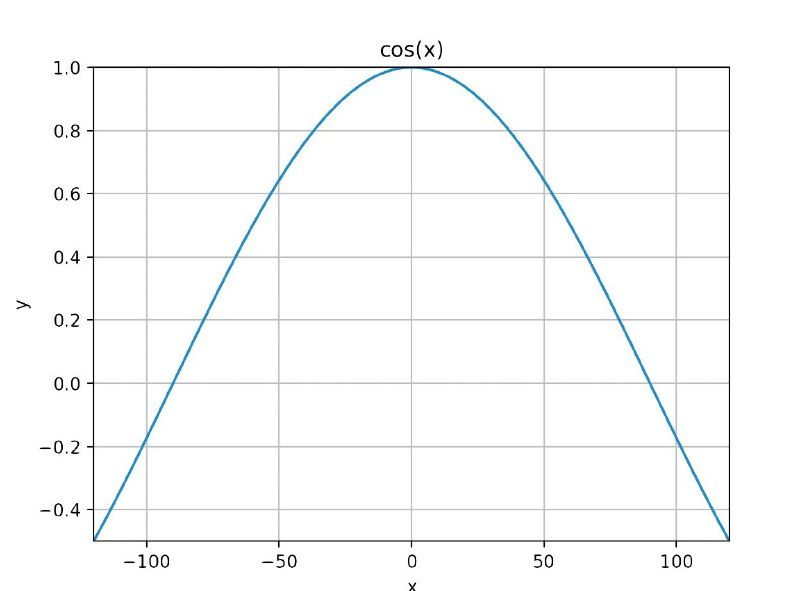
\includegraphics[width=9cm]{81/figs/81_sol.png}
\end{center}

To understand the relation between distributions and vectors recall the definition of correlation: $$\textsf{cor}(x,y) = \frac{\mathsf{covar}(x,y)}{\sqrt{\mathsf{var}(x)\mathsf{var}(y)}}.$$
Let $\Omega$ be the set of all events that define the probability distributions $x$ and $y$ and assume without loss of generality that all elements of $\Omega$ have equal likelihood. We then define $f(x)$ as an $|\Omega|$-dimensional vector as follows:
$$f(x)_{\omega} = x(\omega) - \bar{x}$$ where $x(\omega)$ is the value of distribution $x$ for event $\omega$ and $\bar{x} = \frac{\sum_{\omega' \in \Omega} x(\omega')}{|\Omega|}$ is the average value of distribution $x$. $f(y)$ will be defined similarly. In this setting, the correlation of $x$ and $y$ will be equal to:

$$\begin{aligned}
\textsf{cor}(x,y) =& \frac{\mathsf{covar}(x,y)}{\sqrt{\mathsf{var}(x)\mathsf{var}(y)}}\\
= & \frac{\sum_{\omega \in \Omega} (x(\omega) - \bar{x}) (y(\omega) - \bar{y})/|\Omega|}{\sqrt{(\sum_{\omega \in \Omega} (x(\omega) - \bar{x})^2/|\Omega|)(\sum_{\omega \in \Omega} (x(\omega) - \bar{x}))^2/|\Omega|})} \\
= & \frac{\sum_{\omega \in \Omega} (x(\omega) - \bar{x}) (y(\omega) - \bar{y})}{\sqrt{(\sum_{\omega \in \Omega} (x(\omega) - \bar{x}))^2)(\sum_{\omega \in \Omega} (x(\omega) - \bar{x}))^2)}} \\
= & \frac{\sum_{\omega \in \Omega} f(x)_{\omega} f(y)_{\omega}}{\sqrt{(\sum_{\omega \in \Omega} f(x)_{\omega}^2)(\sum_{\omega \in \Omega} f(y)_{\omega}^2)}} \\
= & \frac{\sum_{\omega \in \Omega} f(x)_{\omega} f(y)_{\omega}}{\sqrt{\sum_{\omega \in \Omega} f(x)_{\omega}^2}\sqrt{\sum_{\omega \in \Omega} f(y)_{\omega}^2}} \\
= &  \frac{f(x)\cdot f(y)}{||f(x)|| \cdot ||f(y)||} \\
= & \cos(\textsf{arc}(f(x), f(y)))
\end{aligned} $$
where $\textsf{arc}(f(x), f(y))$ is the angle between $f(x)$ and $f(y)$.
\end{solution}
